\chapter{Alternativas de desarrollo}\label{alternativas}
En el presente capítulo se ahondará en las distintas alternativas de diseño que existen para el prototipo con los distintos sensores requeridos, además de establecer la comunicación y el envío de la información tomada del paciente. Las etapas para el desarrollo del prototipo constan de: Elección de sistema de procesamiento o unidad central, sensores a utilizar y forma de comunicación inalámbrica.
\section{Plataforma de desarrollo}\label{proce}
Al fabricar un prototipo, el desarrollador debe construir el hardware sobre el cual correrá el software del producto que ha diseñado, por lo que debe tomar componentes de diversos proveedores, integrarlos y hacerlos funcionar como un conjunto. Por esa razón se popularizó el uso de plataformas de desarrollo electrónico.  \\
Por lo general, estas son placas que integran microcontroladores, circuitos y componentes electrónicos que le proporcionan diversas capacidades básicas y a partir de esto se puede evaluar la compatibilidad del diseño tanto en hardware como en software antes de enviar a fabricar el producto final. 

\newpage
\subsection{Arduino}
Arduino es una plataforma de desarrollo de bajo costo que permite crear proyectos de base tecnológica de forma sencilla y barata, que consta de entradas análogas, entradas y salidas digitales, PWM, comunicación serial, etc. 

Uno de los beneficios de Arduino es que provee módulos de desarrollo de bajo costo para trabajar con integrados y estudiar su funcionamiento y prototipado.
Arduino trabaja con una gran variedad microcontroladores AVR que diferencia por modelos dependiendo de las necesidades de proyecto, motivo por el cual varía en precio. 

En primera instancia se puede trabajar con un modelo Arduino UNO que es de bajo costo y permite leer señales análogas y traducirlas en su conversor análogo-digital y dependiendo de las necesidades se puede conseguir otro modelo como Arduino Mega que ofrece mayores prestaciones. 
\subsection{Raspberry}
Raspberry es una computadora de placa reducida (SBC por sus siglas en inglés) de bajo costo, con el objetivo de estimular la enseñanza de ciencias de la computación, no obstante, es de propiedad registrada para poder mantener el control de la 8 plataforma y no se generan excesivas variantes como es el caso de Arduino. El software que usa es open source, aunque es capaz de ejecutar incluso una versión de Windows 10. Por lo mismo su capacidad de procesar señales es mayor y permite ejecutar proyectos más complejos. No se define si es que pueden o no ser usadas en desarrollos comerciales.

\newpage
\subsection{Beaglebone}
Beaglebone black es la última iteración de la serie Beaglebone y su versión pequeña. Esencialmente es similar a Raspberry, diferenciándose en cosas como la capacidad para iniciarse sin la necesidad de instalar ningún sistema operativo ya que tiene memoria integrada, no así Raspberry. Adicionalmente cuenta con una cantidad de entradas sustancialmente mayor, por lo que permite hasta el doble de conexiones que su competencia directa. Como si es no fuera suficiente, la arquitectura del procesador que incluye Beaglebone black permite que rinda hasta el doble de rápido que su contraparte en Raspberry pi. \\
Al igual que su competencia, Beaglebone ofrece mucho mas procesamiento que el necesario por lo que se descarta como una opción para el desarrollo inicial del prototipo, de acuerdo a las necesidades que vayan surgiendo se puede considerar nuevamente como una opción.
\newpage
\section{Sensores}
Hablando con la contraparte de Sistemas Expertos se decidió, a partir de la información que proveen ellos, que las enfermedades  mas comunes son las afecciones cardíacas y también es necesario tener un control de la temperatura de los pacientes a la hora de leer sus signos vitales. \\
Por otra parte se propuso utilizar una IMU para detectar si algún paciente sufre una caída, este con el fin de emitir una alarma para llamar una ambulancia en caso de ser necesario.
\subsection{ECG}
Electrocardiograma o ECG es el proceso de registrar la actividad eléctrica del corazón en un periodo de tiempo usando electrodos directamente en la piel.\\
Lo fundamental será buscar un circuito de desarrollo para realizar una prueba de concepto, en la cual se puedan tomar los datos y manejar.
\subsubsection{DFRobot Heart Rate Monitor Sensor}
El monitor de actividad cardiaca de la empresa DFRobot se usa para medir la actividad electrica del corazón con un integrado AD8232\cite{ad8232} que toma señales análogas de los electrodos y utiliza amplificadores para tener una mejor lectura de los datos.\\
Utilizando un Arduino es posible leer los datos tomados de los electrodos y convertirlos a información digital que puede ser enviada por comunicación serial.\\

\begin{figure}[H]
	\centering
	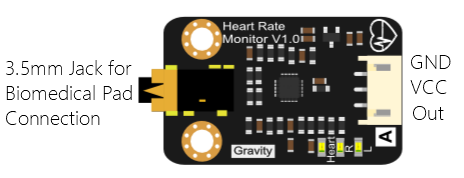
\includegraphics[scale=0.5]{figuras/sensor/ecg/ecg.png}
	\caption{Placa de desarrollo ECG}
	\label{ecg}
\end{figure}

Como se puede observar en la figura \ref{ecg} posee conexión simple para electrodos y salida análoga, lo que permitirá una rápida prueba de concepto para utilizar este integrado en el diseño del dispositivo final. Además este provee filtros que se van a estudiar mas adelante.


\subsubsection{ADS1298}
El integrado ADS1298 de la empresa Texas Instrument ofrece un ECG con 8 amplificadores programables de bajo ruido y 8 conversores Análogo-digital de alta resolución.\\
Utilizado para instrumentación medica y lectura tanto de ECG como EMG (Electromiograma) y EEG (Electroencefalograma).\\
El integrado ADS1298 es una buena opción para un desarrollo de ECG en el futuro de grado médico, pero es de un precio 10 veces mayor al dispositivo de DFRobot por lo que se va a descartar para el prototipo funcional.
\subsection{Temperatura}
Cuando se requiere realizar alguna medición a un paciente siempre es necesario conocer su temperatura corporal que sirve como información complementaria a los profesionales de la salud es por esto que se evaluarán termistores que permitan la lectura de este dato.
\subsubsection{Lilypad Temperature Sensor}
Dentro de la tendencia del hardware abierto, uno de los proyectos más destacados es Lilypad Arduino, un conjunto de piezas electrónicas que se pueden coser a los tejidos para darles interactividad con sensores, luces o sonidos.\\
Entre estos sensores tenemos un sensor de temperatura compuesto por un termistor MCP9700 el cual ofrece una resolución de $\pm2^\circ C.$\\

\newpage
La particularidades que ofrece este sensor es ser de muy bajo costo y a su vez es impermeable por lo que permitiría incorporarlo en el wearable de forma permanente sin dañar la componente.

\begin{figure}[H]
	\centering
	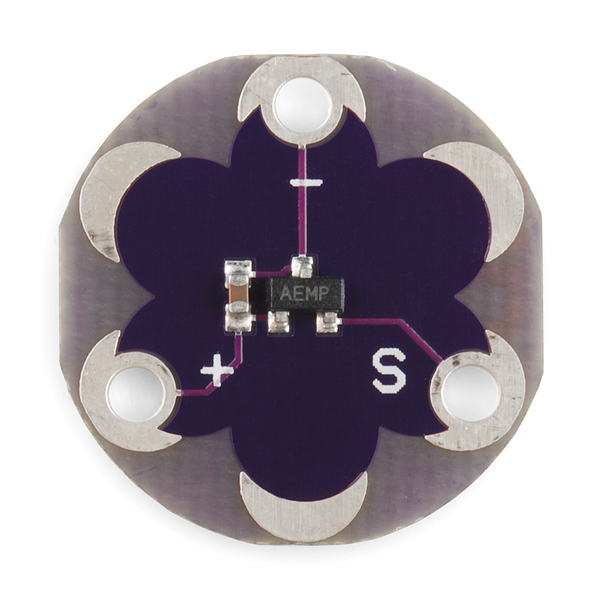
\includegraphics[scale=0.7]{figuras/sensor/t/lilypad.jpg}
	\caption{Sensor de temperatura Lilypad}
	\label{Lilypad}
\end{figure}

Como se puede observar en la figura \ref{Lilypad}, Lilypad ofrece una PCB impermeable con 3 terminales que permiten utilizar un hilo conductor para coser este a la ropa.

\subsubsection{DS18B20}
El sensor DS18B20\cite{temp} es un termómetro digital que ofrece una medida de 9 a 12 bits de resolución. Se comunica mediante el bus 1-Wire (protocolo de comunicación en serie diseñado por Dallas Semiconductor el cual está basado en un maestro y varios esclavos en una sola linea de datos) lo cual permitiría, en caso de ser necesario, incorporar mas sensores para obtener una medida con mayor precisión. 
Este termómetro digital ofrece una resolución de $\pm0.5^\circ C$ y a su vez ofrece un formato impermeable en forma cilíndrica como se observa en la figura \ref{DS18B20}.

\begin{figure}[H]
	\centering
	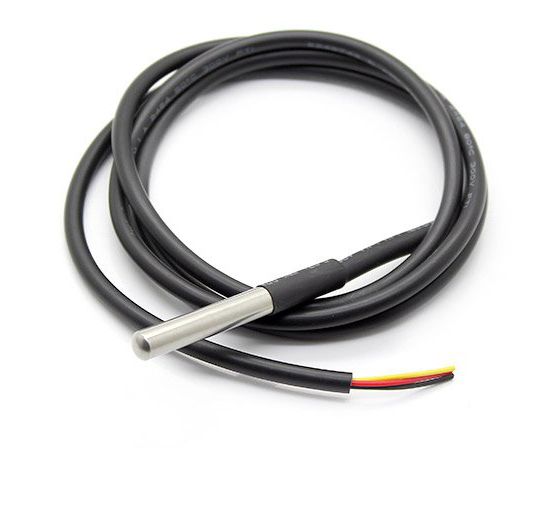
\includegraphics[scale=0.2]{figuras/sensor/t/ds18.jpg}
	\caption{Sensor de temperatura DS18B20}
	\label{DS18B20}
\end{figure}

\subsection{Ritmo Respiratorio}
Para medir el ritmo respiratorio, sensor que la contraparte pidió estudiar utilizando una tela conductora, se consideró el uso de la tela conductiva MedTex, la cual entrega un valor de resistividad en ohms en su estado en reposo y este varía dependiendo de su estiramiento.\\

\begin{figure}[H]
	\centering
	
\includegraphics[scale=0.5]{figuras/tela/medtex.jpg}
	\caption{Tela Conductiva MedTex}
	\label{medtex}
\end{figure}

Para estudiar la factibilidad de la tela conductiva que se puede observar en la figura \ref{medtex} se cortó una tira de un tamaño $20x2 [cm]$ en estiramiento cero sobre una banda elástica que luego fue cosida como cinturón de pecho. Una vez colocada en cada extremo de la tela conductiva se colocó un caimán conectado a su vez a un multitester que permitía visualizar variaciones de la resistividad de la tela a partir de su estiramiento. 

\newpage
\begin{table}[H]
	\centering
	\begin{tabular}{| c | c | c |}
		\hline
		\multicolumn{1}{|c|}{\textbf{Resistencia en reposo [$\Omega$]}}&
		\multicolumn{1}{c|}{\textbf{Resistencia en estiramiento [$\Omega$]}}&
		\multicolumn{1}{|c|}{\textbf{\% de variación)}}\\ \hline
		$4.8$  & $4.6$  & $0.1420$  \\ \hline
		$4.7$  & $4.5$ & $0.1421$ \\ \hline
		$4.8$ & $4.7$  & $0.0722$  \\ \hline
	\end{tabular}
	\caption{Valores resistencia Tela MedTex en Pectorales}
	\label{tablatex1}
\end{table}

\begin{table}[H]
	\centering
	\begin{tabular}{| c | c | c |}
		\hline
		\multicolumn{1}{|c|}{\textbf{Resistencia en reposo [$\Omega$]}}&
		\multicolumn{1}{c|}{\textbf{Resistencia en estiramiento [$\Omega$]}}&
		\multicolumn{1}{|c|}{\textbf{\% de variación)}}\\ \hline
		$4.7$  & $4.6$  & $0.0699$  \\ \hline
		$4.7$  & $4.6$ & $0.0699$ \\ \hline
		$4.6$ & $4.5$  & $0.0723$  \\ \hline
	\end{tabular}
	\caption{Valores resistencia Tela MedTex en Plexo}
	\label{tablatex2}
\end{table}

\begin{table}[H]
	\centering
	\begin{tabular}{| c | c | c |}
		\hline
		\multicolumn{1}{|c|}{\textbf{Resistencia en reposo [$\Omega$]}}&
		\multicolumn{1}{c|}{\textbf{Resistencia en estiramiento [$\Omega$]}}&
		\multicolumn{1}{|c|}{\textbf{\% de variación)}}\\ \hline
		$4.7$  & $4.6$  & $0.0699$  \\ \hline
		$4.8$  & $4.7$ & $0.0722$ \\ \hline
		$4.7$ & $4.5$  & $0.1421$  \\ \hline
	\end{tabular}
	\caption{Valores resistencia Tela MedTex en Estomago}
	\label{tablatex3}
\end{table}

Se puede observar en las tablas \ref{tablatex1}, \ref{tablatex2} y \ref{tablatex3} las variaciones de resistencias no son constantes ni regulares, el mismo estiramiento a veces no producía la misma variaciones de resistencia. Además por mínimas variaciones en el movimiento también habían variaciones que arruinaban la medición, por lo que esta alternativa no sería viable para medir el ritmo respiratorio.

\subsection{Unidad de movimiento inercial (IMU)}
Una unidad de movimiento inercial o IMU (del inglés inertial measurement unit), es un dispositivo electrónico que mide la aceleración, inclinación y las fuerzas gravitacionales, usando una combinación de acelerómetros y giroscopios.
\subsubsection{MPU-9250}
El integrado MPU-9250 es un modulo multi-chip que consiste en 2 integrados en un empaquetado QFN. Este provee un giroscopio de 3 ejes y un acelerómetro de 3 ejes.
Este chip provee tres conversores análogo-digital de 16 bits para digitalizar las salidas del giroscopio, acelerómetro y giroscopio de manera independiente.\\
Sparkfun provee una PCB de desarrollo para realizar pruebas como se muestra en la imagen \ref{imu1}.

\begin{figure}[H]
	\centering
	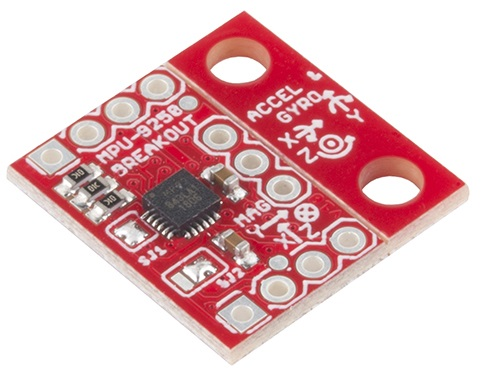
\includegraphics[scale=1.5]{figuras/sensor/imu/imu1.jpg}
	\caption{IMU Sparkfun MPU-9250}
	\label{imu1}
\end{figure}

Es importante destacar la orientación indicada por el fabricante al momento de diseñar el equipo electrónico que son predefinidas como se puede ver en el caso de la figura \ref{imu1} en la cual se muestran los ejes X, Y y Z tanto para el acelerómetro como para el giroscopio. 
\newpage
Como se observa en la figura \ref{imu11} se muestra además de los ejes de aceleración también las coordenadas de navegación (roll, pitch, yaw). 

\begin{figure}[H]
	\centering
	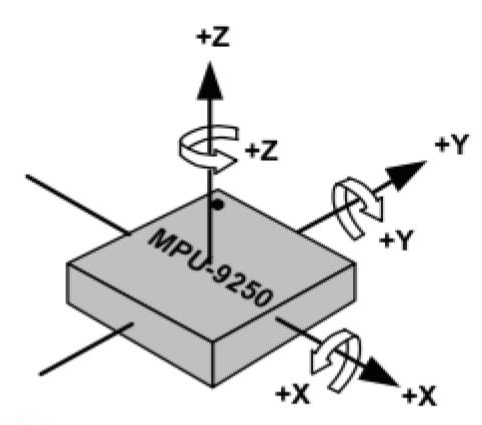
\includegraphics[scale=0.5]{figuras/sensor/imu/imu11.jpg}
	\caption{Ejes IMU MPU-9250}
	\label{imu11}
\end{figure}

\section{Comunicación}
Para el proyecto se consideran distintas alternativas de conexión, las cuales deben seguir ciertos aspectos relevantes según las especificaciones del dispositivo a implementar. 


\begin{enumerate}
	\item \textbf{Alta disponibilidad:}
	Se requiere que la tecnología a emplear permita establecer conexiones a lo largo del tiempo, presentando pocas o de preferencia nulas desconexiones o incapacidades de conexión.
	\item \textbf{Gran cobertura:}
	Considerando la envergadura inicial del proyecto, Chile, es de vital importancia que la tecnología a utilizar permita generar conexiones en la mayor parte del territorio nacional.
	\item \textbf{Bajo costo:}
	Dentro de los requerimientos del proyecto se encuentra el desarrollo e implementación a bajo costo de la solución final, por tanto la tecnología de comunicación a emplear debe seguir esta directriz para ser seleccionada.
	\item \textbf{Baja complejidad:}
	Considerando que el dispositivo en cuestión debiera ser lo más autónomo y sencillo de configurar, es relevante considerar tecnologías de comunicación que no requieran de complejas operaciones para su uso e implementación.
	\item \textbf{Escalabilidad:}
	Si bien es un aspecto dependiente de los anteriores requerimientos, es relevante considerarlo por separado como la medida que representa la capacidad de atender una gran cantidad de conexiones (usuarios en definitiva). 
\end{enumerate}

En base a lo anterior, se hace un análisis rápido de diferentes alternativas que podrían utilizarse en el proyecto:

\begin{enumerate}
	\item \textbf{Antenas de RF:}\cite{RF}
	Comunicación generada en las bandas situadas entre los 3 kilohercios (KHz) y 300 Gigahercios (GHz). Esta tecnología incluye distintas otras tecnologías como las redes celulares, pero en este apartado se especifica el uso de bandas no utilizadas por esta y otras tecnologías. Permitiendo una conexión directa de antena a antena a una frecuencia específica a determinar.
	
	\item \textbf{Comunicación satelital:}\cite{satelite}
	Comunicación  por medio de ondas electromagnéticas transmitidas gracias a la presencia en el espacio de satélites artificiales situados en órbita alrededor de la Tierra. Dentro de esta tecnología se pueden encontrar dos grandes clasificaciones: Satélites activos y Satélites pasivos, los cuales se diferencian por la amplificación o de las señales antes de ser reenviadas a la Tierra, respectivamente.
	
	\item \textbf{Redes Wi-Fi:}\cite{wifi}
	También llamada WLAN (Wireless lan, red inalámbrica) o estándar IEEE 802.11, es una de las tecnologías de comunicación inalámbrica mediante ondas más utilizada hoy en día. Existen distintas variantes de este estándar de comunicación, entre los que se destacan 802.11g y 802.11n, por su uso actual en dispositivos comerciales.
	
	\item \textbf{Redes celulares:}\cite{celular}
	Consiste en una red de celdas cada una con su propio transmisor, conocidas como estación base. Ampliamente utilizadas en la actualidad, lográndose encontrar hasta 7 compañías distintas que ofrecen sus servicios en Chile: Movistar, Entel, WOM, Claro, Virgin, VTR, SIMPLE.
	\begin{enumerate}
		\item \textbf{Comunicación directa:}
		Tipo de comunicación en donde el dispositivo posee la capacidad de conectarse, registrarse y hacer uso completo de la infraestructura proporcionada por distintas compañías.
		
		\item \textbf{Comunicación indirecta:}
		Tipo de comunicación con la cual el dispositivo requiere de un paso intermedio de comunicación para generar la conexión a la red requerida, para este paso se puede destacar el uso de Bluetooth para la comunicación con otro dispositivo con la capacidad de conectarse de forma directa a las redes celulares.
	\end{enumerate}	
\end{enumerate}	

Luego de caracterizar las distintas tecnologías disponibles para su uso en el proyecto, se procede a analizar sus cualidades en función de las 4 especificaciones anteriores: 

\begin{table}[H]
	\centering
	\begin{tabular}{| c | c | c | c | c | c |}
		\hline
		\multicolumn{1}{|c|}{\textbf{Tecnología}}&
		\multicolumn{1}{c|}{\textbf{Disponibilidad}}&
		\multicolumn{1}{|c|}{\textbf{Cobertura}}&
		\multicolumn{1}{|c|}{\textbf{Costo}}&
		\multicolumn{1}{|c|}{\textbf{Complejidad}}&
		\multicolumn{1}{|c|}{\textbf{Escalabilidad}}\\ \hline
		Antenas RF  & Alta  & Baja & Alta & Alta & Baja \\ \hline
		Satelital  & Alta & Alta & Alta & Alta & Baja\\ \hline
		Wi-Fi & Alta & Baja  & Bajo & Media & Alta\\ \hline
		Celular directa & Alta  & Alta  & Medio & Baja & Alta\\ \hline
		Celular indirecta & Alta  & Alta/Baja & Bajo & Media & Alta/Median\\ \hline
	\end{tabular}
	\caption{Comparativa tecnologías / requerimientos}
	\label{tablacompara_telecomunicaciones}
\end{table}

A raíz de lo anterior se destaca el uso de tecnologías con redes celulares por su lineamiento con el proyecto. La tecnología Wi-Fi se descarta por ser de baja cobertura (pensando a nivel nacional) y esto a su vez ser un ámbito crítico para el proyecto. A continuación se presentan alternativas para la plataforma Arduino en torno a las tecnologías ya mencionadas.

\subsection{Celular directa: GPRS/GSM shield}
Para integrar conexión a redes celulares en el dispositivo es necesario considerar un GPRS shield compatible con socket xbee.\\ GPRSBee cumple con los requerimientos a un precio no menor (aproximadamente 36.000 CLP). 
Se puede observar en la figura \ref{gprs} el módulo disponible para desarrollo.

\begin{figure}[H]
	\centering
	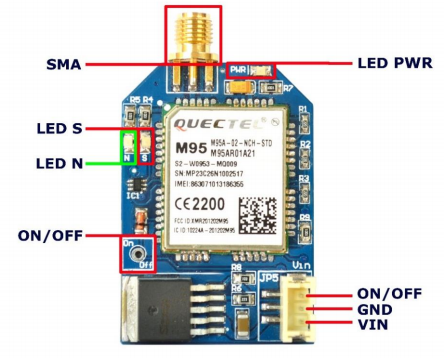
\includegraphics[scale=0.8]{figuras/com/gprs.png}
	\caption{Modulo GPRSBee}
	\label{gprs}
\end{figure}

Cabe destacar que para poder utilizar este módulo es necesario incluir una antena que se puede ver en la figura \ref{antena}

\begin{figure}[H]
	\centering
	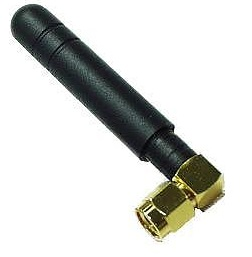
\includegraphics[scale=0.5]{figuras/com/antena.jpg}
	\caption{Antena GPRSBee}
	\label{antena}
\end{figure}

Al considerar este módulo se puede concluir que es incompatible con el diseño del wearable ya que la antena es muy grande (aproximadamente $57.40[mm]$ ) lo que sería molesto en el dispositivo final. Otro punto en contra de este módulo es el alto costo y el consumo energía que lo hace incompatible con la autonomía que se desea.

\subsection{Celular indirecta: Bluetooth BLE shield}
Para integrar Bluetooth en el dispositivo se considera un BLEBee el cual ofrece Bluetooth versión 4.1 y comunicación UART mediante un puerto XBEE. \\
El shield Bluetooth posee un módulo RN4020\cite{RN4020} el cual ofrece una antena para la comunicación en su misma placa lo que facilita el diseño como se puede observar en la figura \ref{bt}.

\begin{figure}[H]
	\centering
	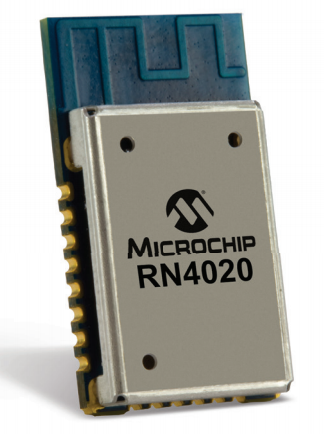
\includegraphics[scale=0.5]{figuras/com/rn4020.png}
	\caption{Bluetooth RN4020}
	\label{bt}
\end{figure}

Es importante destacar que para mejorar el diseño, el fabricante recomienda dejar expuesta la antena y se destaca la comunicación UART para las configuraciones futuras del sistema.

\newpage

\section{Conclusiones}
En esta sección, tomando en cuenta las opciones vistas en el mismo capítulo, se seleccionarán las primeras componentes a utilizar para el prototipo funcional y para realizar la prueba de concepto con lo que se va a basar el proyecto.
\subsection{Plataforma de desarrollo}
Para la plataforma de desarrollo se va a escoger trabajar con Arduino ya que este posee distintas versiones con distintos costos, los cuales son menores que Raspberry o Beaglebone. Además cabe destacar que el sistema que se quiere desarrollar es toma de datos y envío de información por lo que no se va a requerir tanto procesamiento. Arduino cubre las necesidades en su versión UNO con un microcontrolador ATMega328p, en caso de necesitar uno de mayor capacidad se puede optar por un Arduino Mega.
\subsection{Electrocardiograma}
Para el sensor de electrocardiograma se utilizará el monitor de actividad cardíaca de DFRobot, esto debido a que es la única opción que se puede conseguir en el país para no retrasar el desarrollo. Este sensor es de muy bajo costo (alrededor de 19.500 CLP en MCIElectronics).
El integrado ADS1298 es una buena opción como una mejora para una segunda iteración del diseño para mejorar la señal que se puede obtener debido a que este posee mayor tolerancia al ruido. Se debe destacar esta última opción debido a que se debe encargar directamente desde Texas Instruments y esto puede tomar mucho tiempo.
\subsection{Temperatura}
En primera instancia se va a utilizar el sensor Lilypad ya que este está diseñado específicamente para wearables además de que utiliza un hilo conductor para unir sus terminales con la alimentación y la toma de datos. Este sensor tiene un valor aproximado de 3.790 CLP.\\
Dependiendo de los resultados obtenidos en la primeras pruebas se va a evaluar la segunda alternativa de utilizar el DS18B20 el cual tiene un valor aproximado de 5.900 CLP.
\subsection{IMU}
Al buscar las alternativas que existen en el país, todas las opciones de desarrollo usan distintas placas de desarrollo pero utilizan el mismo sensor MPU-9250 por lo que se va a utilizar la placa de Sparkfun MPU-9250 luego de tener el prototipo funcional con los primeros sensores de electrocardiograma y temperatura. Esta placa de desarrollo tiene un valor aproximado de 12.500 CLP.
\subsection{Comunicación}
Entre las alternativas mencionadas, se opta por utilizar en primera instancia el GPRS shield, el cual posee un costo aproximado de 43.980 CLP.
Cabe mencionar que en una segunda instancia se utilizaría el chip RN4020, el cual posee un precio aproximado de 20.000 CLP.\\
Si bien el costo es menor, es relevante la complejidad que agrega la segunda opción (al agregar un actor como lo puede ser un teléfono inteligente), es este criterio el que nos lleva a priorizar de esta forma la elección en este punto.